To ensure the security and accessibility of the system, we have implemented various authentication mechanisms, including:
\begin{itemize} 
\item \textbf{Login}: Users can securely login using their credentials to access the system's features and functionalities.
\begin{figure}[H]
    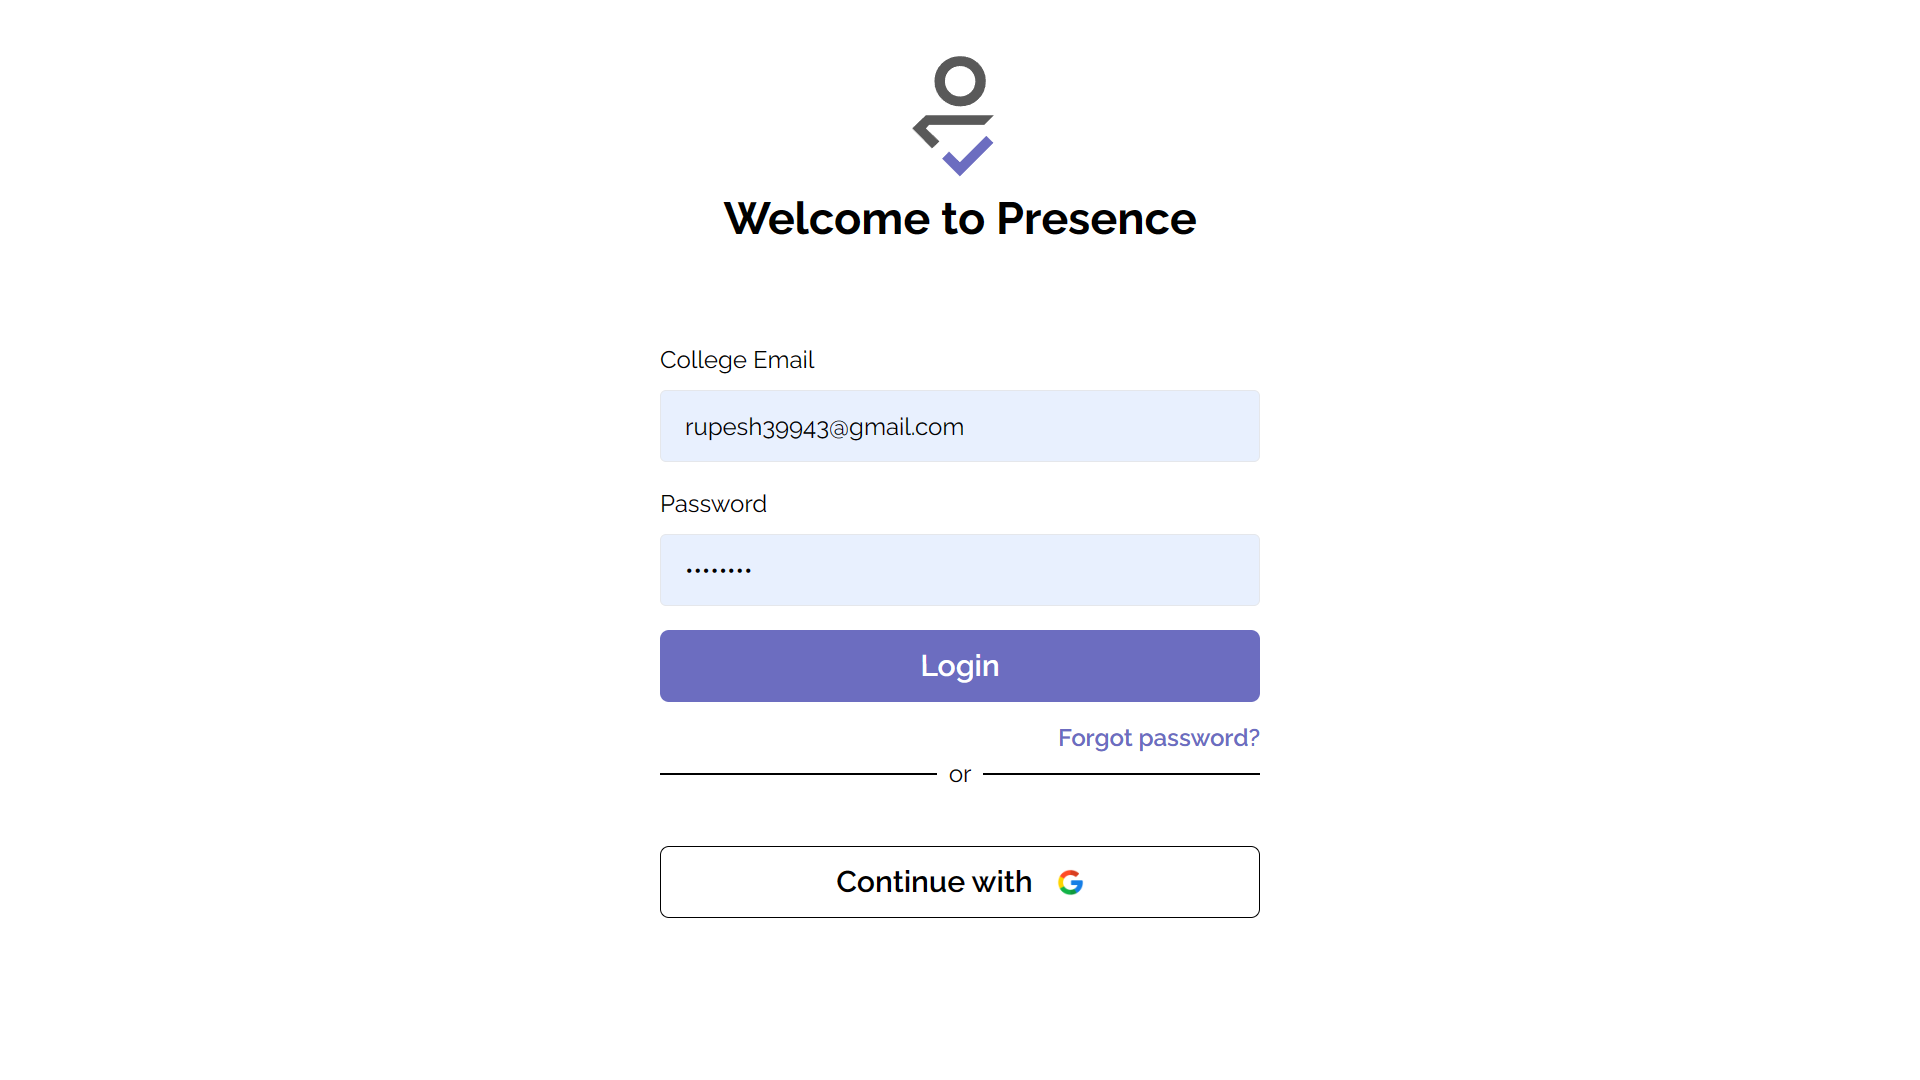
\includegraphics[width=\linewidth]{figures/login.png}
    \centering
    \caption{Login form for both users and admin}
\end{figure}
\item \textbf{Login with Google}: Users have the option to authenticate themselves using their Google accounts, providing a convenient and streamlined login experience.
\begin{figure}[H]
    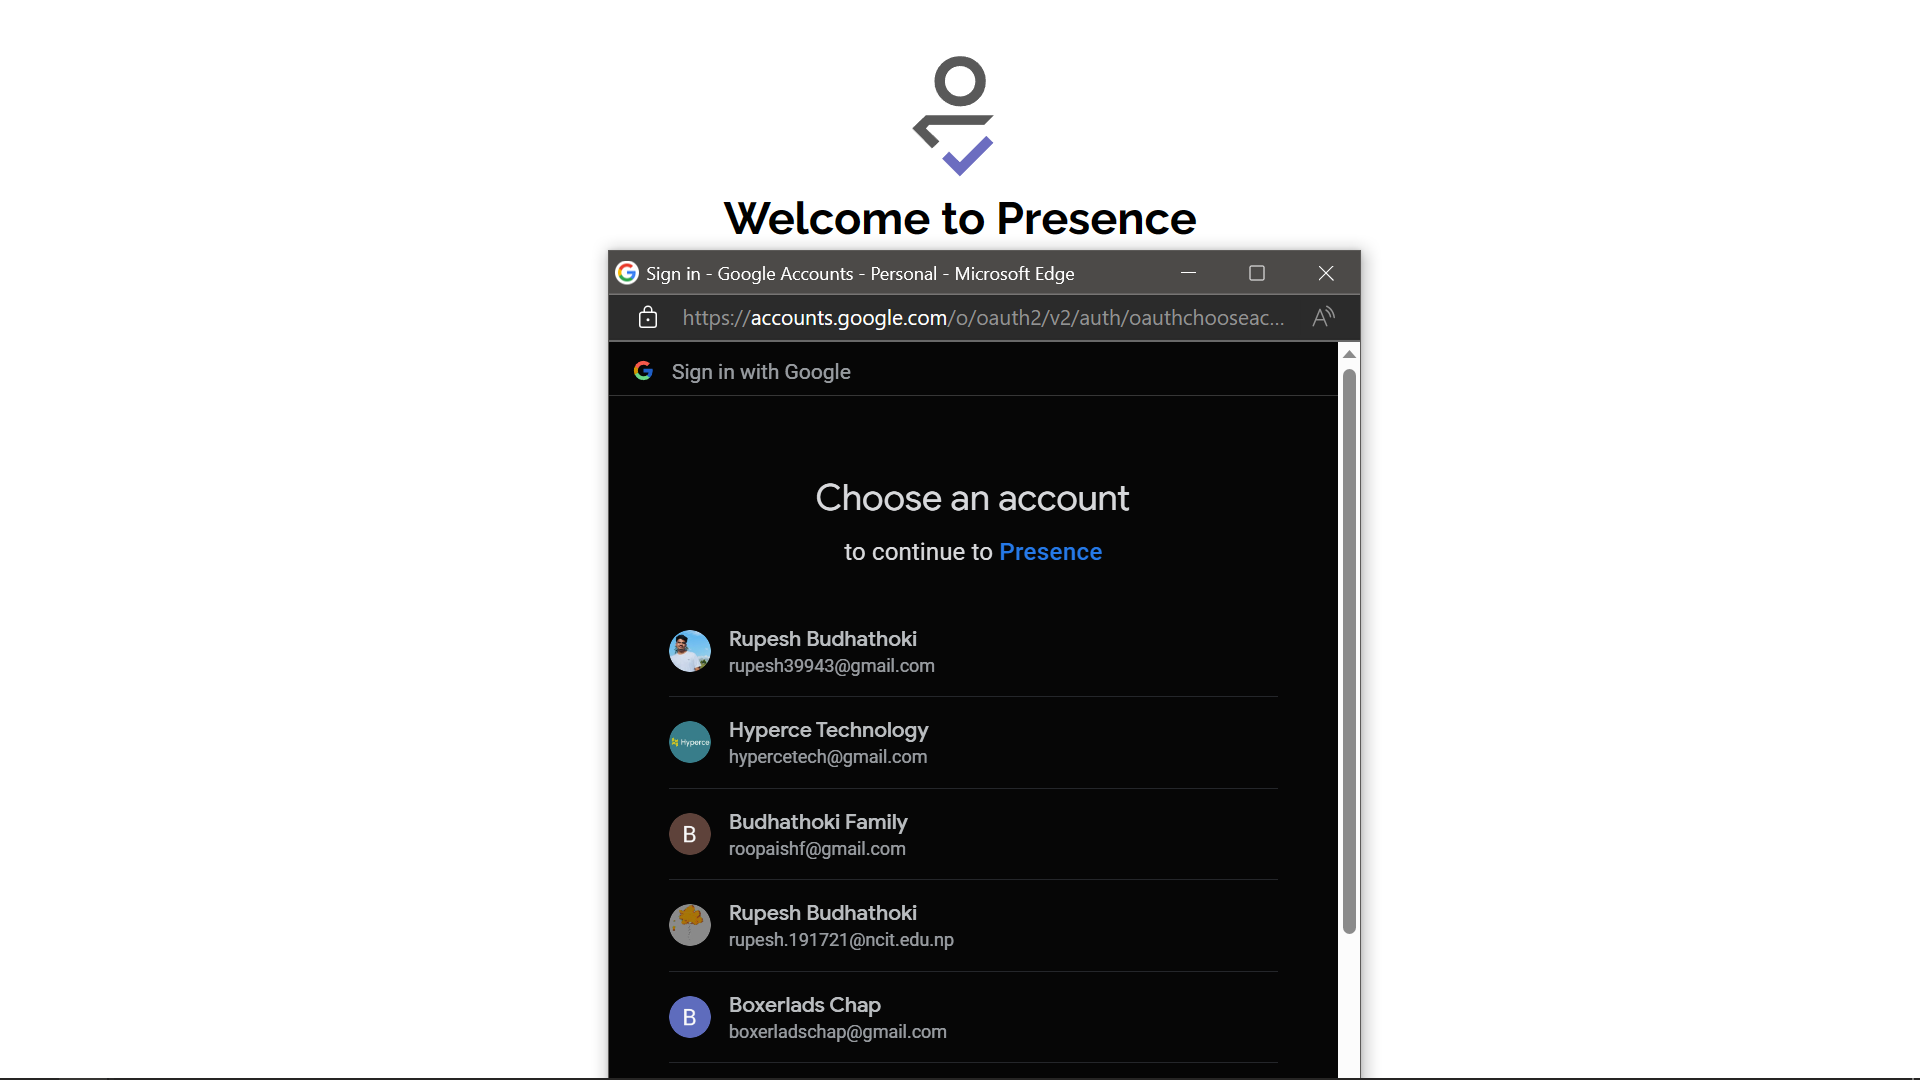
\includegraphics[width=\linewidth]{figures/login-with-google.png}
    \centering
    \caption{Login with Google functionality}
\end{figure}
\item \textbf{Forgot Password}: In the event of a forgotten password, a password recovery mechanism allows users to reset their passwords securely.
\begin{figure}[H]
    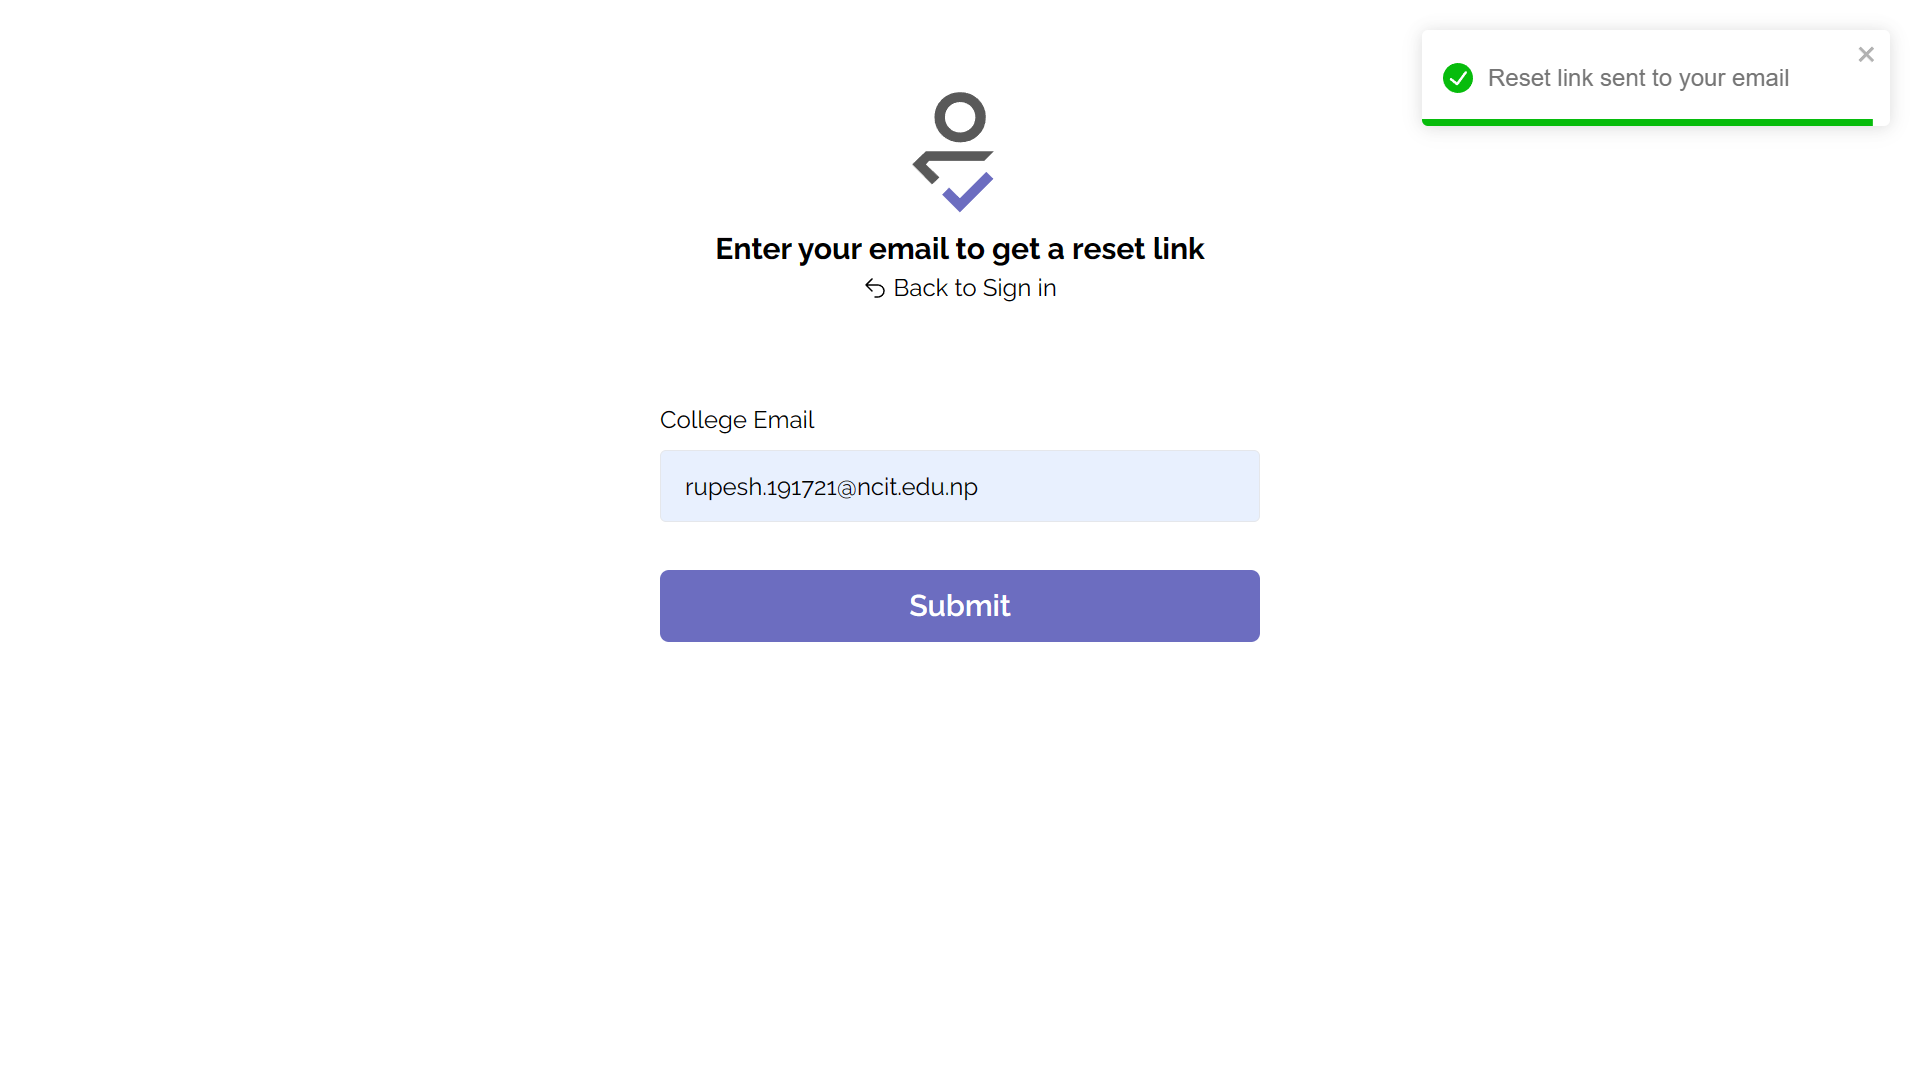
\includegraphics[width=\linewidth]{figures/forgot-password.png}
    \centering
    \caption{Login with google functionality}
\end{figure}
\item \textbf{Reset Password}: Users can initiate the password reset process and set a new password to regain access to their accounts.
\begin{figure}[H]
    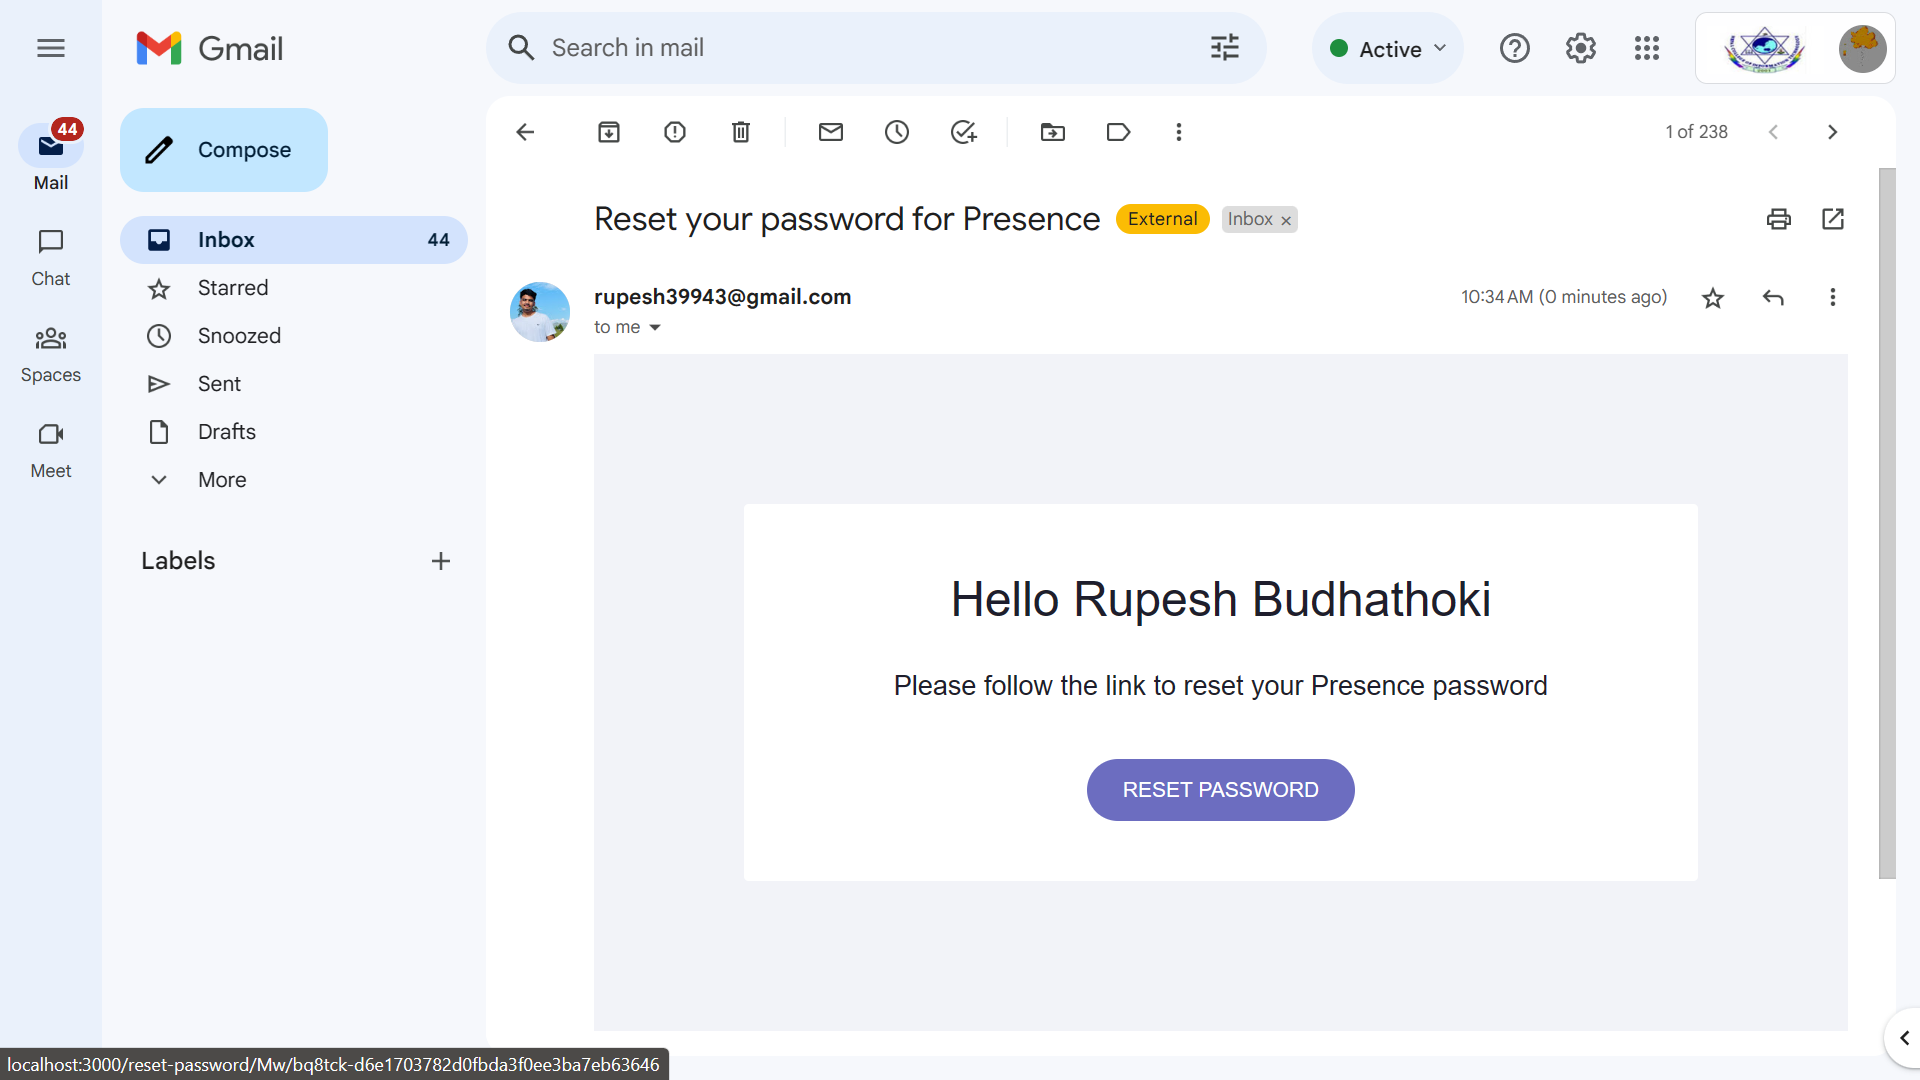
\includegraphics[width=\linewidth]{figures/reset-pw-email.png}
    \centering
    \caption{Reset Password Email}
\end{figure}
\begin{figure}[H]
    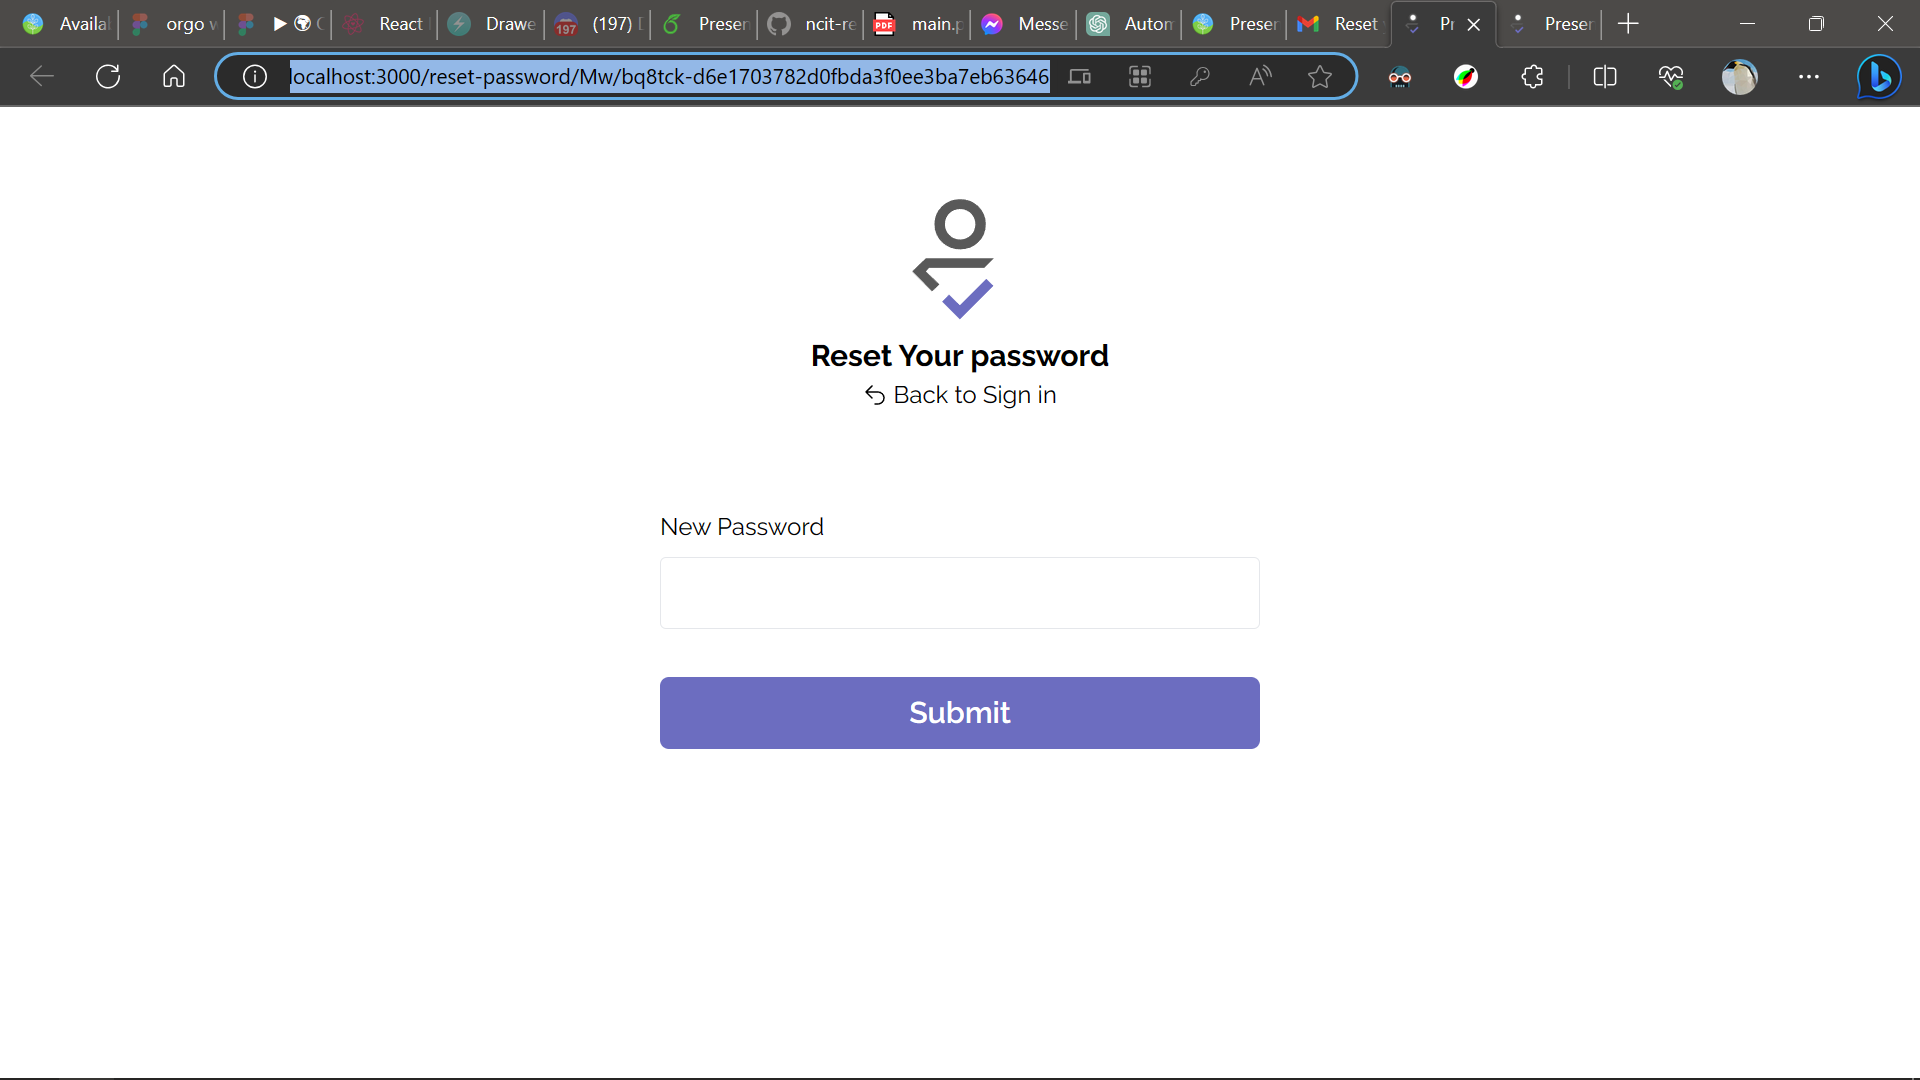
\includegraphics[width=\linewidth]{figures/reset-pw.png}
    \centering
    \caption{Reset password}
\end{figure}
\end{itemize}

Key Features for Students:
\begin{itemize} 
\item \textbf{Image Submission}: Students can submit their images to be used for facial recognition and attendance tracking.
\begin{figure}[H]
    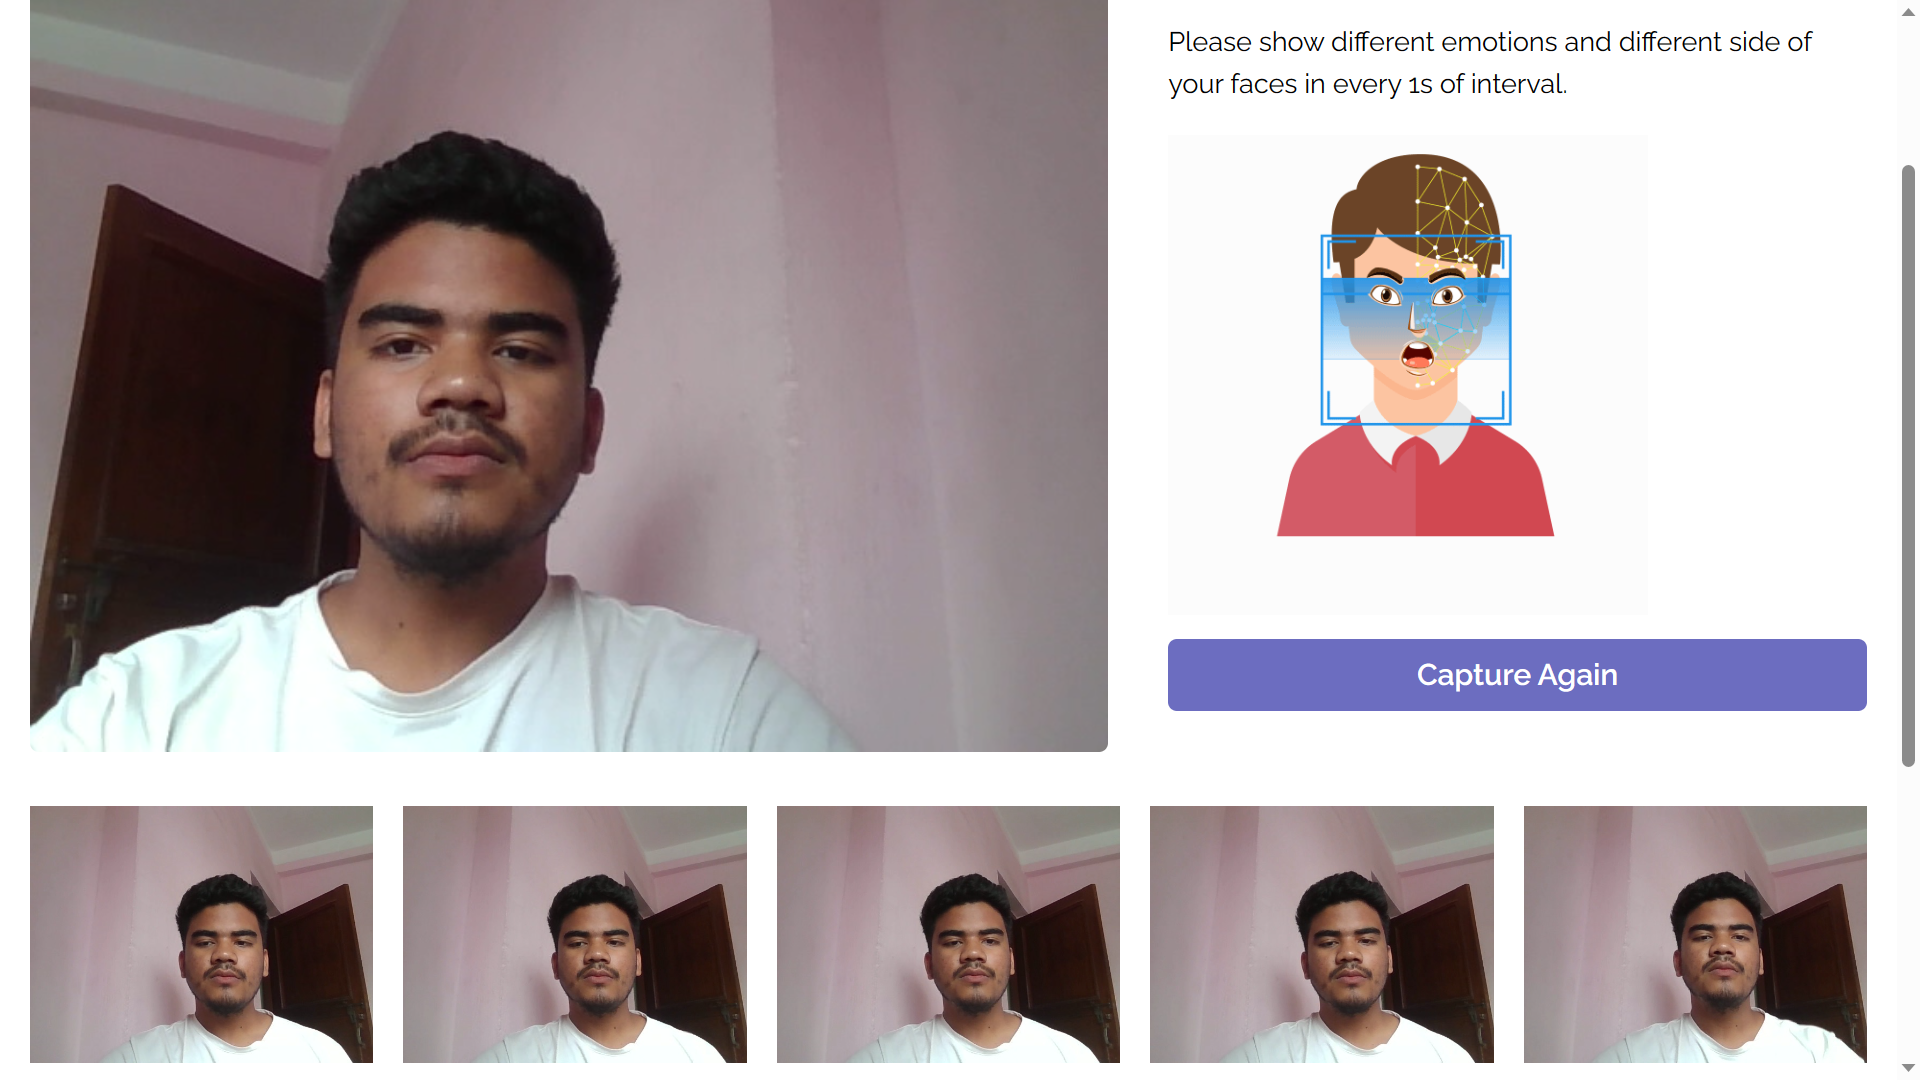
\includegraphics[width=\linewidth]{figures/submit-images.png}
    \centering
    \caption{Image submission form}
\end{figure}
\item \textbf{Attendance Tracking}: Students have access to view their attendance records, providing insights into their attendance patterns and history.
\begin{figure}[H]
    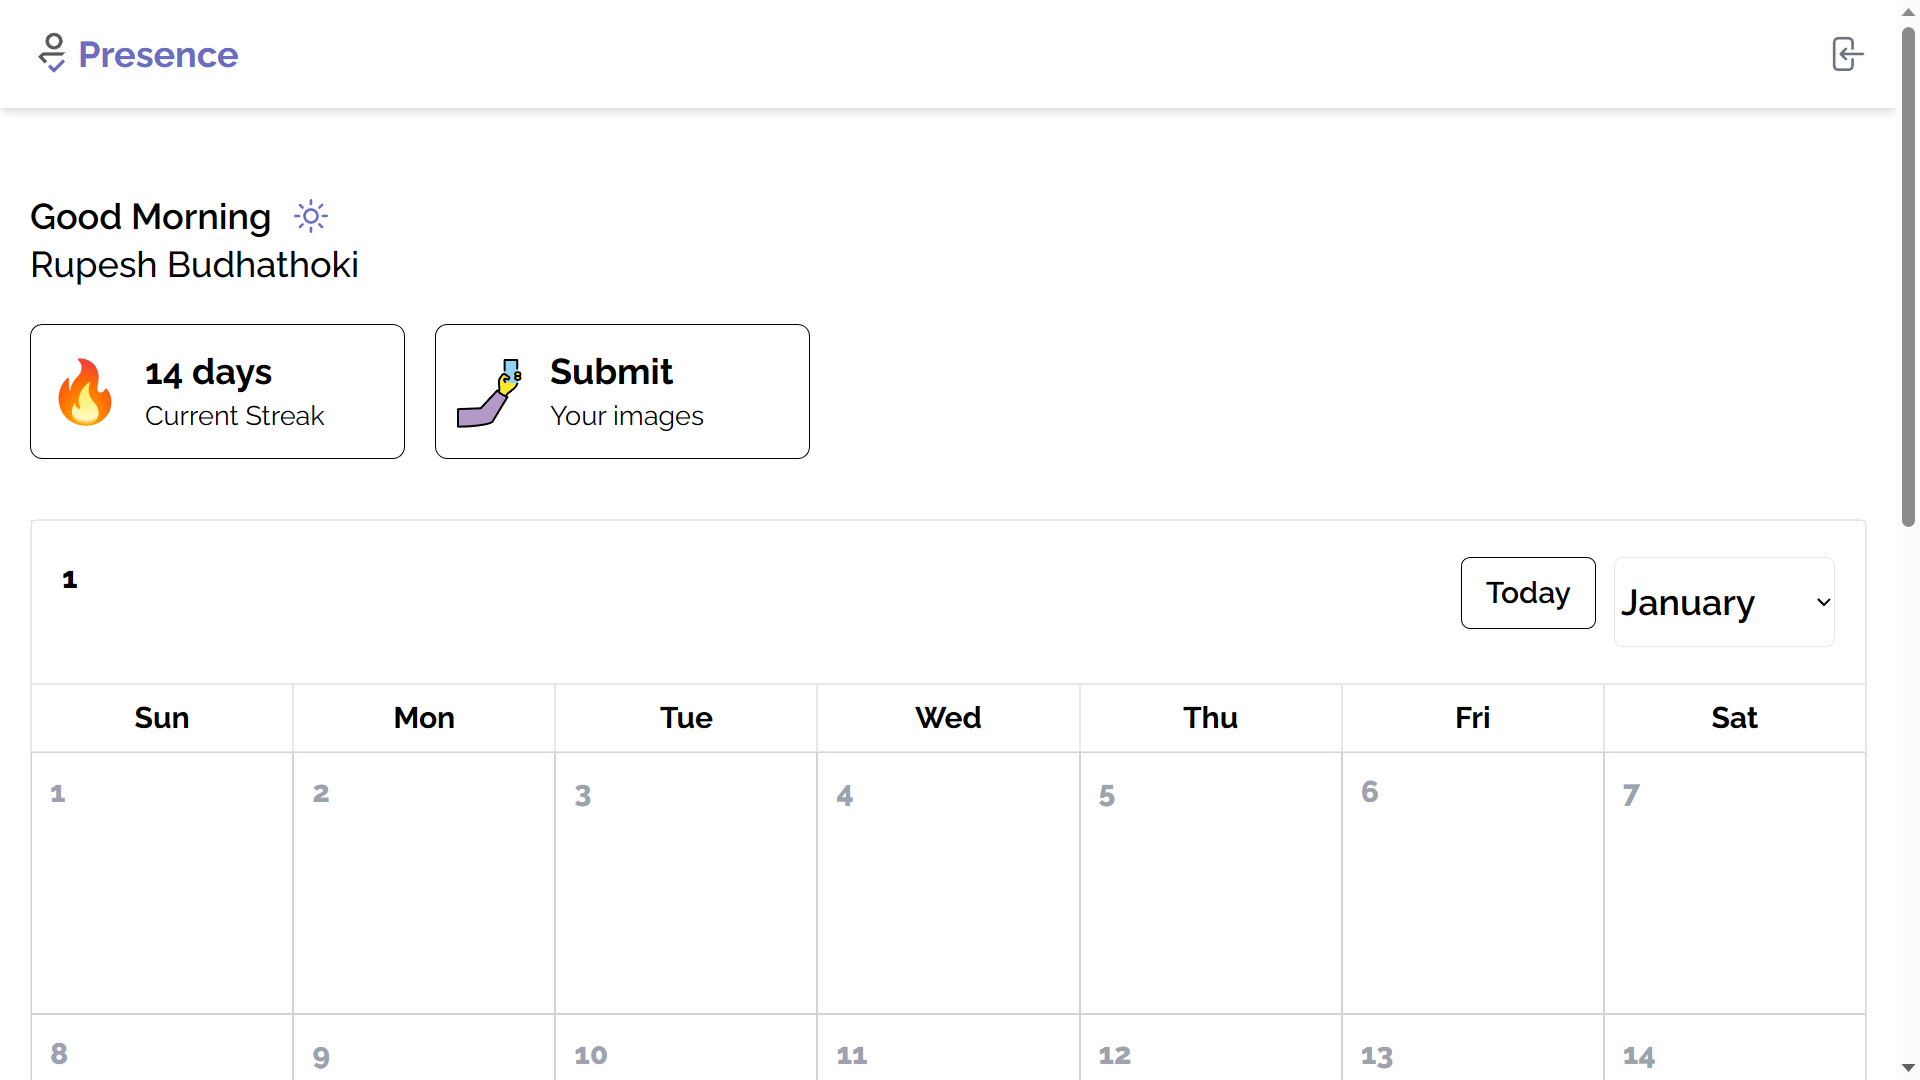
\includegraphics[width=\linewidth]{figures/student-dash.png}
    \centering
    \caption{Student dashboard}
\end{figure}
\end{itemize}


Key Features for Authorities:
\begin{itemize} 
\item \textbf{Student Management}: Authorities can add new students to the system, maintaining an up-to-date database of enrolled individuals.
\begin{figure}[H]
    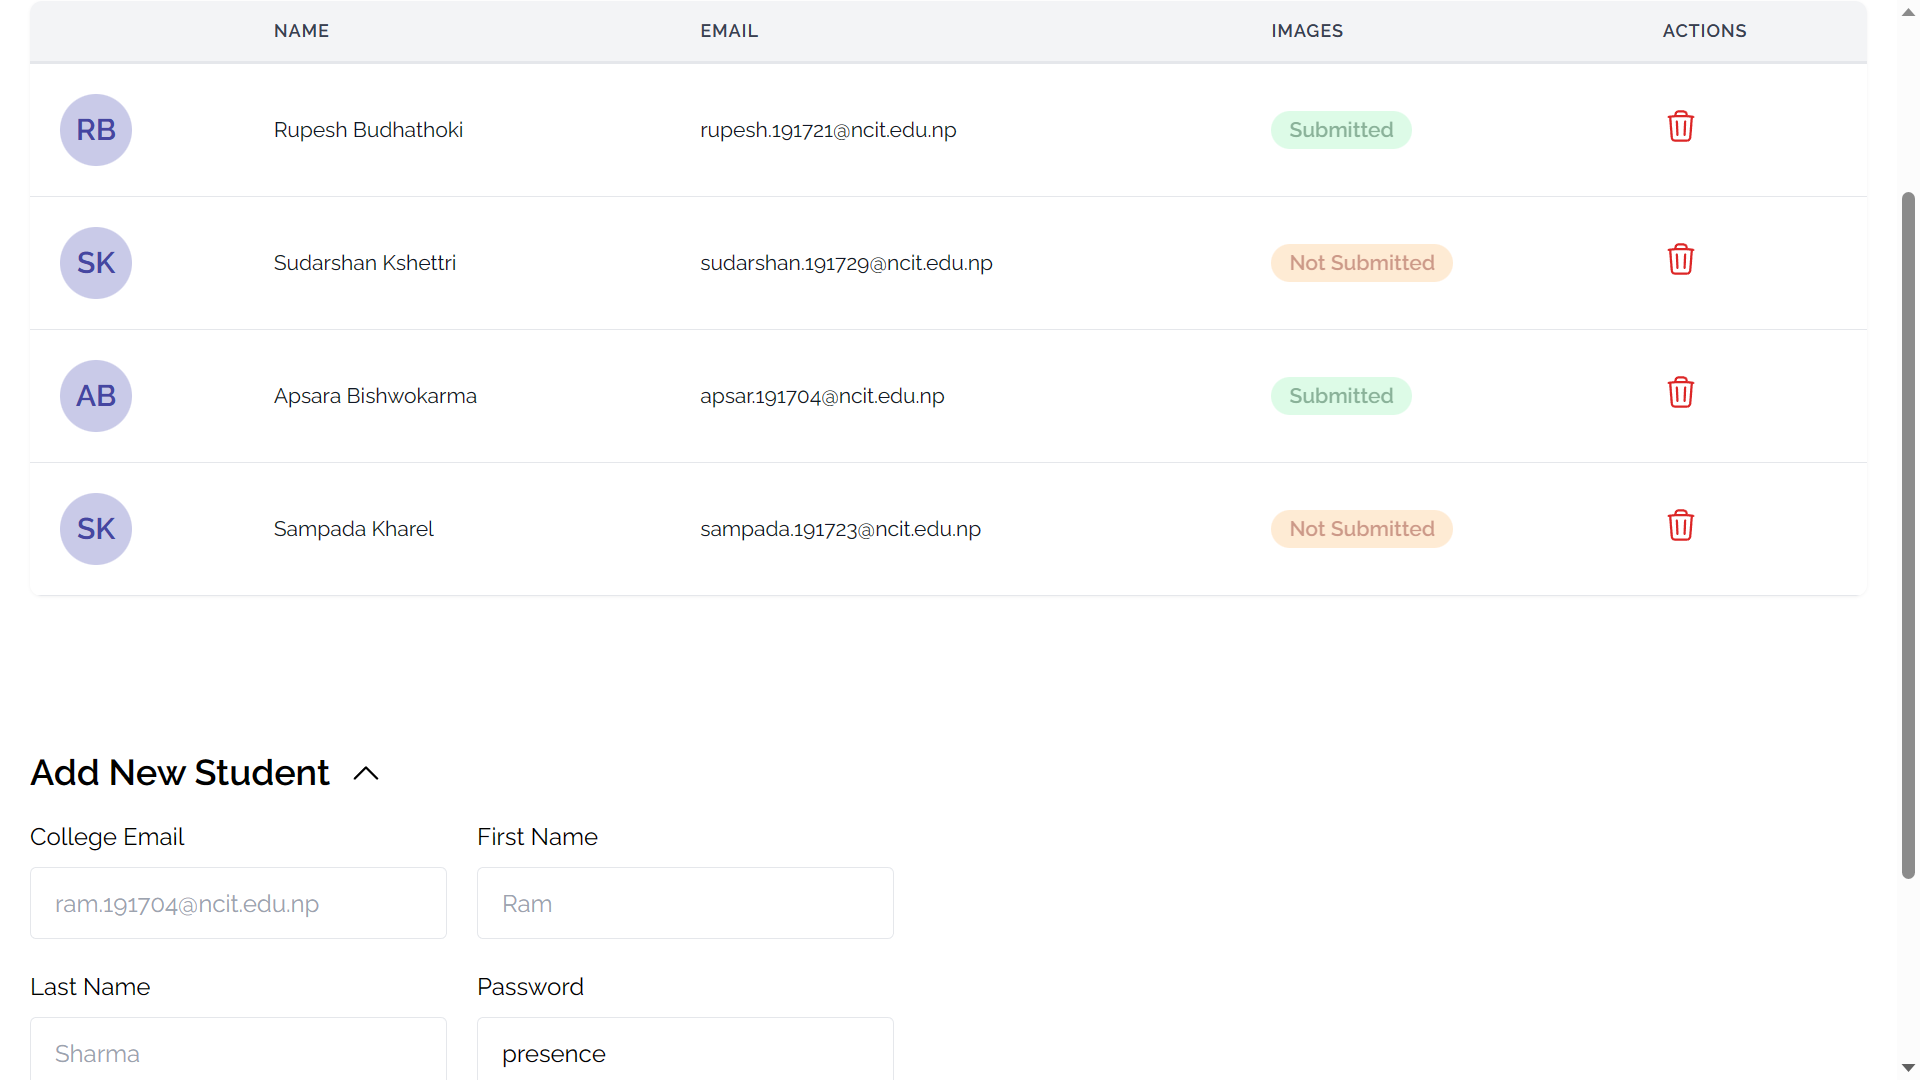
\includegraphics[width=\linewidth]{figures/students-list.png}
    \centering
    \caption{Student Management}
\end{figure}
\item \textbf{Model Training}: Authorities have the ability to train the facial recognition model using images submitted by students, ensuring accurate and reliable attendance detection.
\begin{figure}[H]
    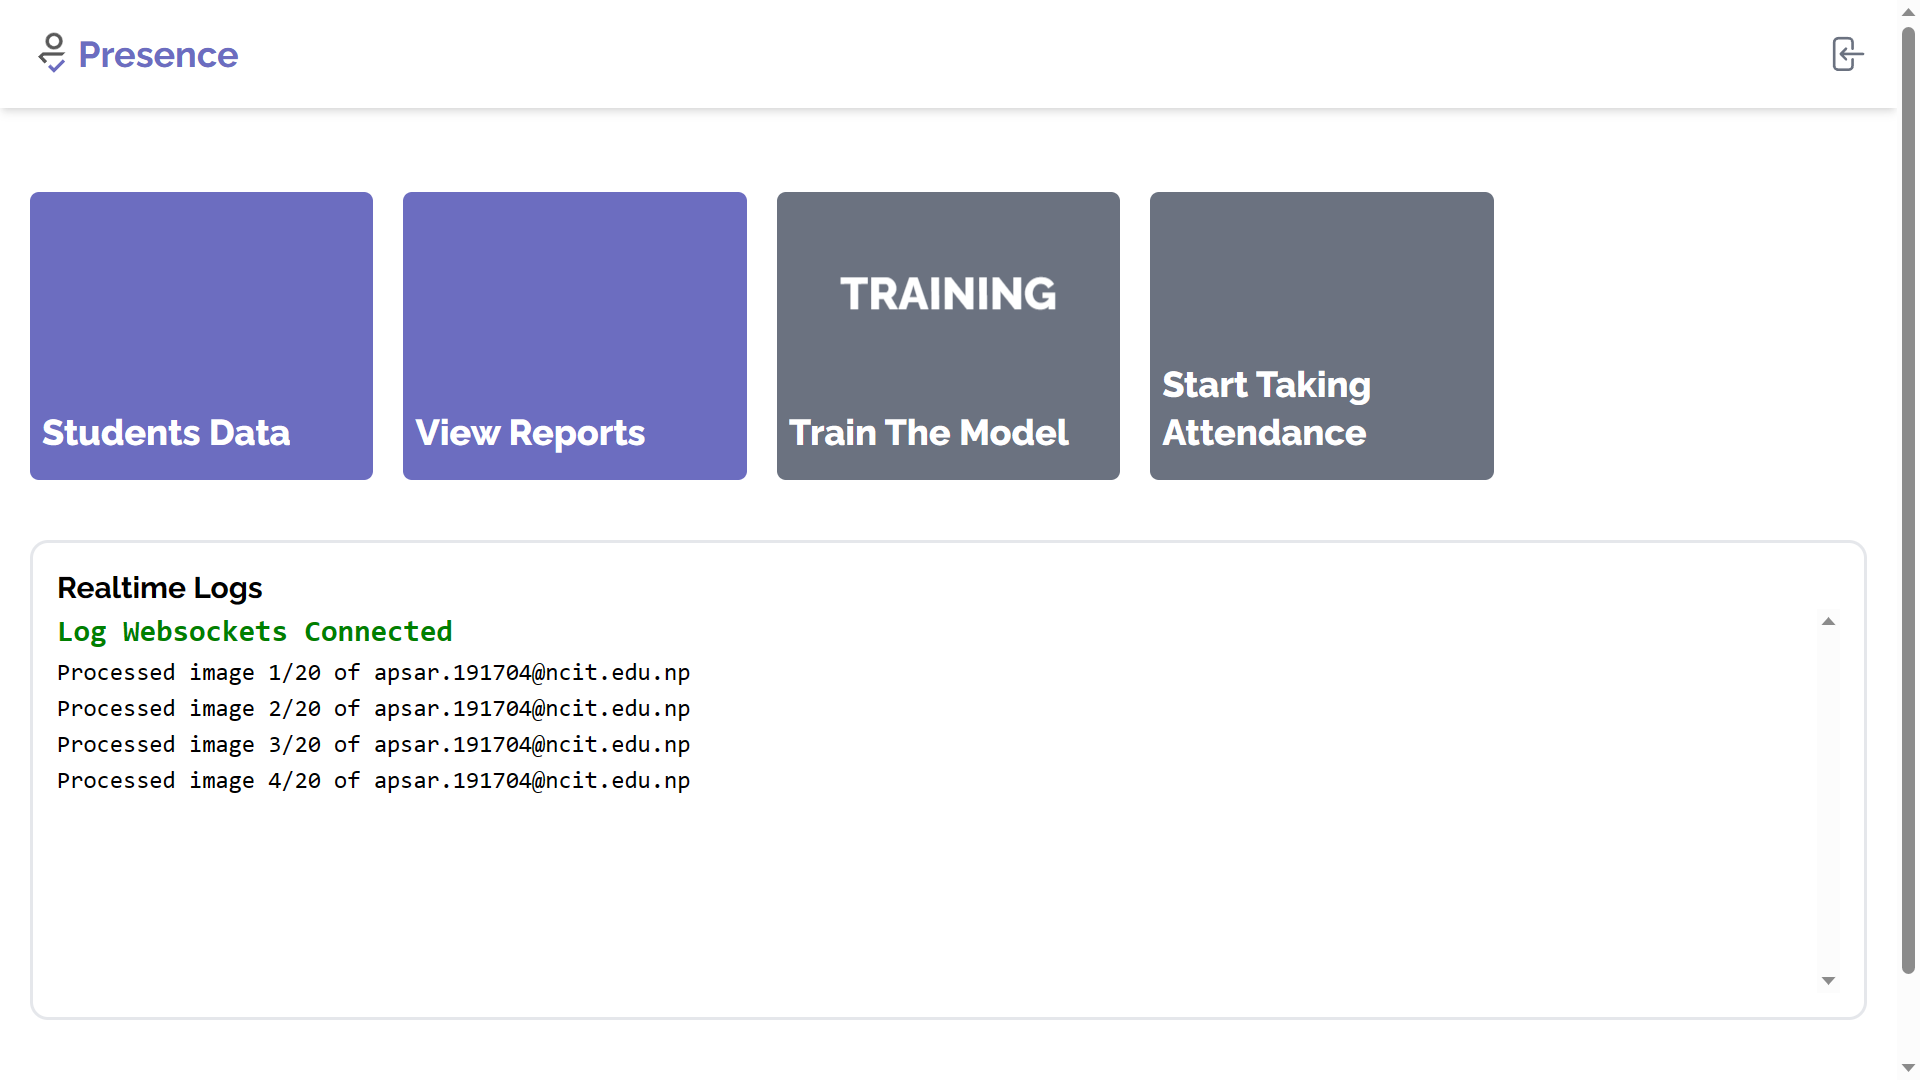
\includegraphics[width=\linewidth]{figures/training.png}
    \centering
    \caption{Training model with images submitted by students}
\end{figure}
\item \textbf{Real-time Attendance}: Authorities can initiate the real-time attendance process, enabling the system to mark attendance as students are recognized.
\begin{figure}[H]
    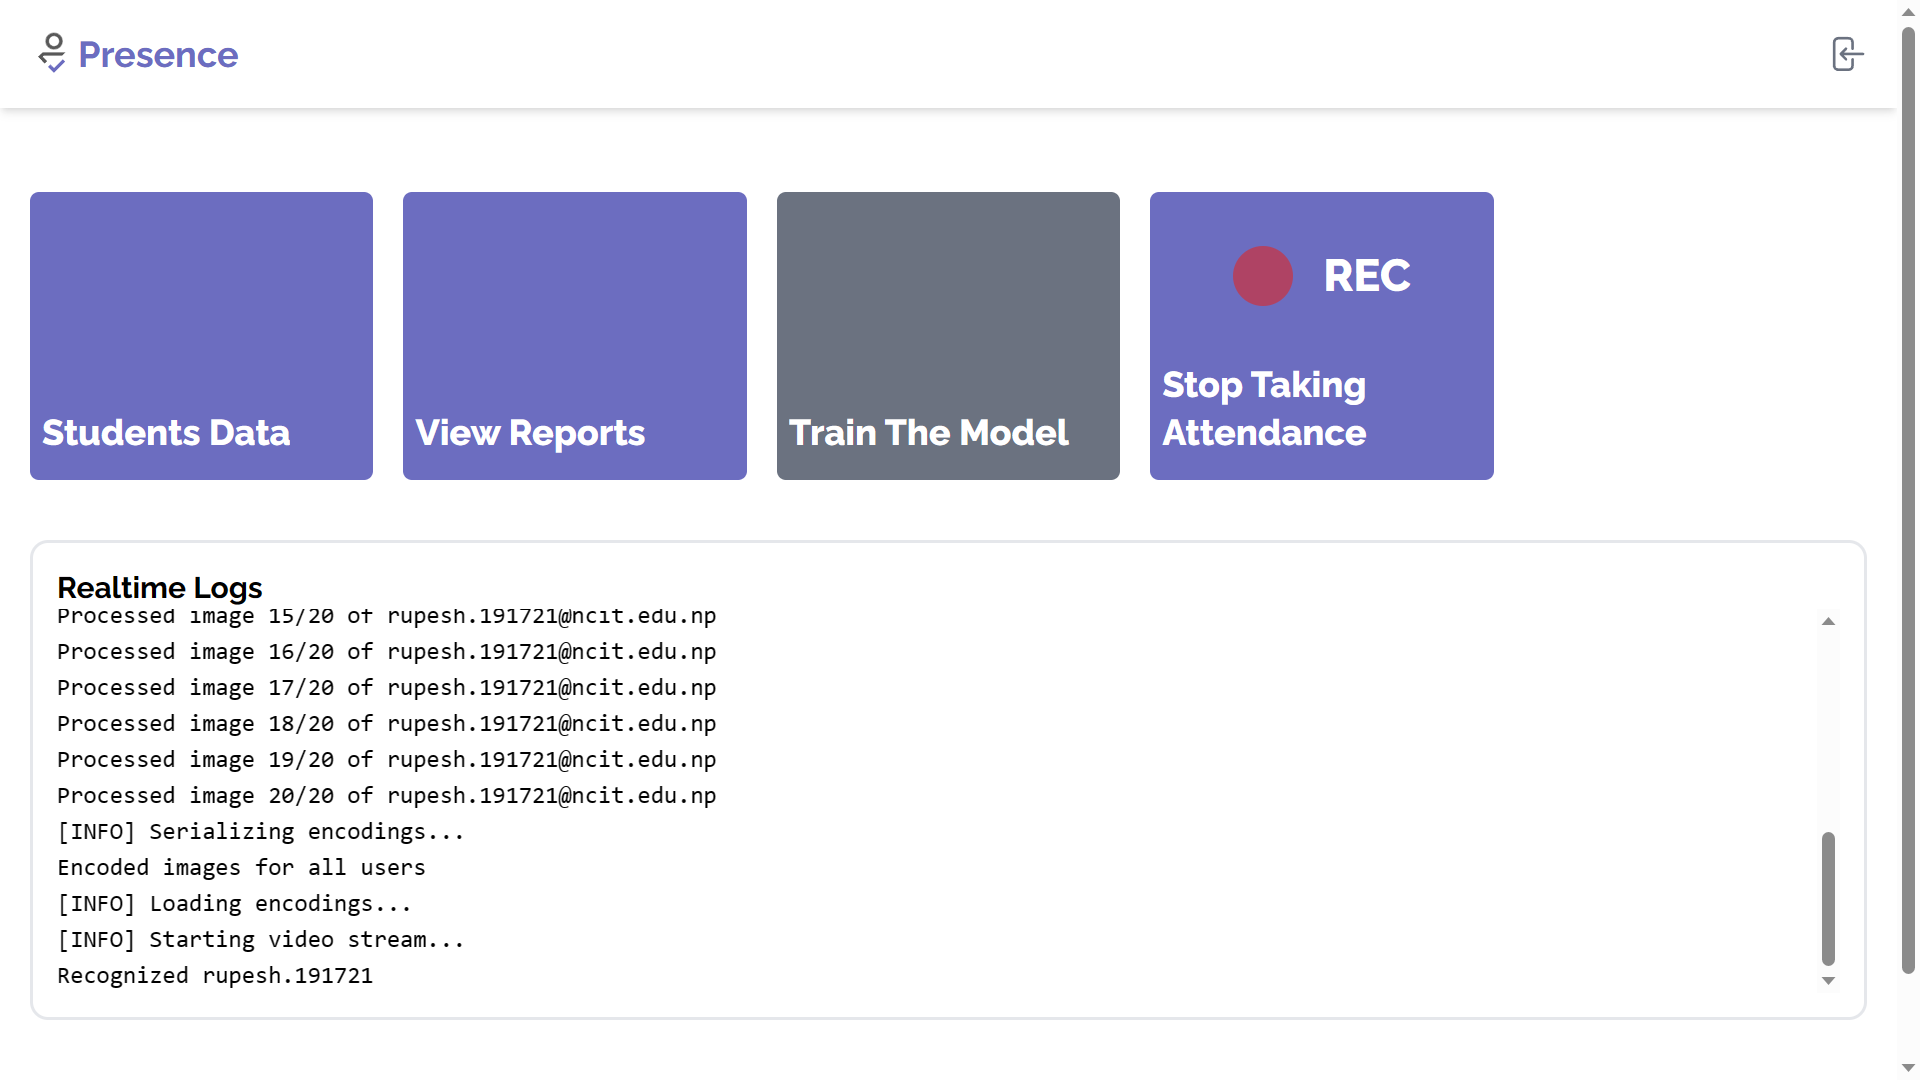
\includegraphics[width=\linewidth]{figures/taking-attendance.png}
    \centering
    \caption{Realtime attendance log}
\end{figure}
\begin{figure}[H]
    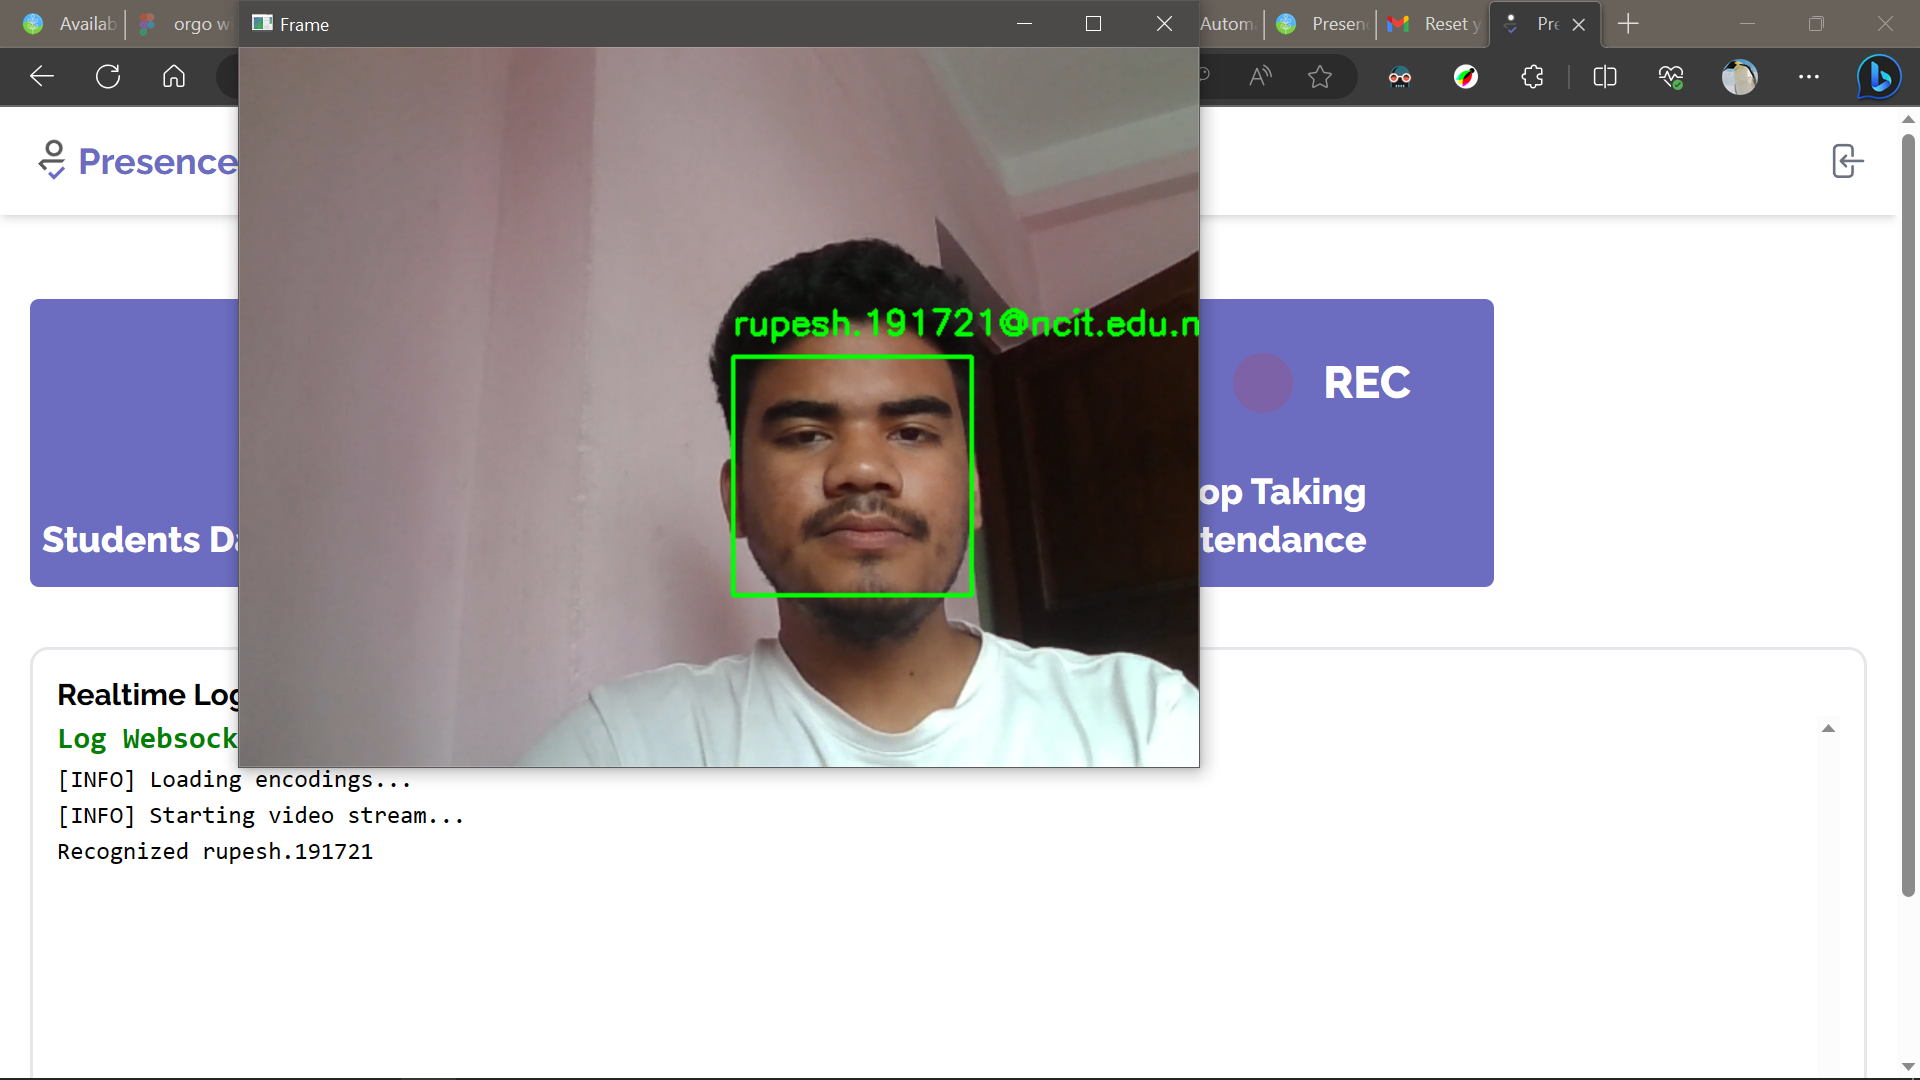
\includegraphics[width=\linewidth]{figures/python-cam.png}
    \centering
    \caption{Realtime attendance from cam}
\end{figure}

\item \textbf{Student Calendar}: Student attendance status.
\begin{figure}[H]
    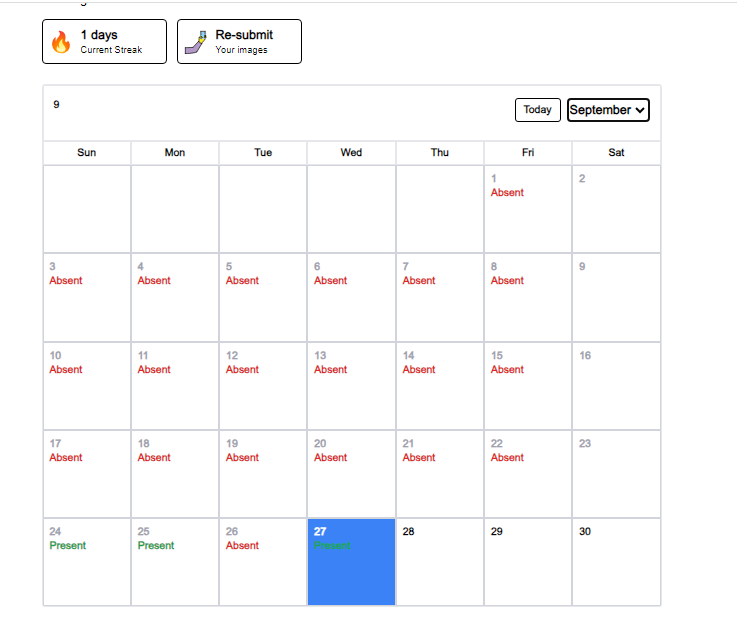
\includegraphics[width=\linewidth]{figures/student-calendar.png}
    \centering
    \caption{Student Calendar}
\end{figure}

\item \textbf{Encode Faces}: Code snippet to encode faces and make a pickle file.

\begin{minted}{python}

@user_passes_test(lambda u: u.is_superuser)
def encode_images(request):
    dataset_path = 'datasets'
    encodings_path = 'encodings.pickle'
    channel_layer = get_channel_layer()

    async_to_sync(channel_layer.group_send)(
        'status_group',
        {
            'type': 'status_message',
            'message': "encoding_images"
        }
    )

    if not os.path.exists(dataset_path):
        return JsonResponse({'success': False, 'message':
        'Dataset directory not found'}, status=400)

    image_paths = list(paths.list_images(dataset_path))

    known_encodings = []
    known_names = []

    for (i, image_path) in enumerate(image_paths):
        name = os.path.basename(os.path.dirname(image_path))
        image = cv2.imread(image_path)
        rgb = cv2.cvtColor(image, cv2.COLOR_BGR2RGB)

        boxes = face_recognition.face_locations(rgb)
        encodings = face_recognition.face_encodings(rgb, boxes)

        for encoding in encodings:
            known_encodings.append(encoding)
            known_names.append(name)

        async_to_sync(channel_layer.group_send)(
            'log_group',
            {
                'type': 'log_message',
                'message': f"""Processed image
                {i+1}/{len(image_paths)} of {name}"""
            }
        )

    async_to_sync(channel_layer.group_send)(
        'log_group',
        {
            'type': 'log_message',
            'message': f"[INFO] Serializing encodings..."
        }
    )
    data = {"encodings": known_encodings, "names": known_names}
    with open(encodings_path, "wb") as f:
        f.write(pickle.dumps(data))

    async_to_sync(channel_layer.group_send)(
        'log_group',
        {
            'type': 'log_message',
            'message': "Encoded images for all users"
        }
    )
    async_to_sync(channel_layer.group_send)(
        'status_group',
        {
            'type': 'status_message',
            'message': "none"
        }
    )

    return JsonResponse({'success': True})


stop_stream = False
\end{minted}

\item \textbf{Take Attendance}: Code snippet to take attendance of users.

\begin{minted}{python}

@user_passes_test(lambda u: u.is_superuser)
@csrf_exempt
def take_attendance(request):
    global stop_stream


    if request.method == 'POST':
        json_data = json.loads(request.body)
        display_video = json_data.get('display_video') or False
        model = json_data.get('model') or 'hog'
        day = date.today().day
        month = date.today().month
        year = date.today().year
        
    # return JsonResponse({'success': month, 'message': 'month'},status=200)
         

        if Attendance.objects.filter(day=day, month=month, year=year).exists():
            return JsonResponse({'success': day, 'message': """Attendance 
            for today is already taken"""}, status=200)

        channel_layer = get_channel_layer()
        dataset_path = 'datasets'
        encodings_path = 'encodings.pickle'
        image_paths = list(paths.list_images(dataset_path))

        if not os.path.exists(dataset_path):
            return JsonResponse({'success': False, 'message': """Dataset 
            directory not found"""}, status=400)

        # Load the known faces and embeddings
        async_to_sync(channel_layer.group_send)(
            'log_group',
            {
                'type': 'log_message',
                'message': "[INFO] Loading encodings..."
            }
        )
        async_to_sync(channel_layer.group_send)(
            'status_group',
            {
                'type': 'status_message',
                'message': "taking_attendance"
            }
        )
        data = pickle.loads(open(encodings_path, "rb").read())
        # Initialize the video stream and allow the camera sensor
        # to warm up
        async_to_sync(channel_layer.group_send)(
            'log_group',
            {
                'type': 'log_message',
                'message': "[INFO] Starting video stream..."
            }
        )
        vs = VideoStream(src=0).start()
        time.sleep(2.0)

        detected_users = []
        names = []
        # get all users and make a list of {name, email}
        attendance_stream = {
            'present_users': [],
            'absent_users': [],
        }
        users = User.objects.all()
        for user in users:
            attendance_stream['absent_users'].append({
                'name': user.first_name + ' ' + user.last_name,
                'email': user.email
            })

        today = date.today()
        attendance_queryset = Attendance.objects.filter(
            day=today.day, month=today.month, year=today.year)

        # Loop over frames from the video file stream
        while True:
            if stop_stream:
                break
            # Grab the frame from the threaded video stream
            frame = vs.read()

            # Convert the input frame from BGR to RGB 
            # then resize it to have
            # a width of 750px (to speed up processing)
            rgb = cv2.cvtColor(frame, cv2.COLOR_BGR2RGB)
            rgb = imutils.resize(frame, width=750)
            r = frame.shape[1] / float(rgb.shape[1])
            # Detect the (x, y)-coordinates of the bounding boxes
            # corresponding to each face in the input frame, then compute
            # the facial embeddings for each face
            boxes = face_recognition.face_locations(rgb, model=model)
            encodings = face_recognition.face_encodings(rgb, boxes)
            names = []

            # Loop over the facial embeddings
            for encoding in encodings:
                # Attempt to match each face in the 
                # input image to our known encodings
                matches = face_recognition.compare_faces(
                    data["encodings"], encoding)
                name = "Unknown"
                # Check to see if we have found a match
                if True in matches:
                    # Find the indexes of all matched faces 
                    # then initialize a
                    # dictionary to count the
                    # total number of times each face
                    # was matched
                    matchedIdxs = [i for (i, b) in enumerate(matches) if b]
                    counts = {}
                    # Loop over the matched indexes and 
                    # maintain a count for
                    # each recognized face face
                    for i in matchedIdxs:
                        name = data["names"][i]
                        counts[name] = counts.get(name, 0) + 1
                    # Determine the recognized face with the largest number
                    # of votes (note: in the event of an unlikely tie Python
                    # will select the first entry in the dictionary)
                    name = max(counts, key=counts.get)

                    confidence = (counts[name] / len(matchedIdxs)) * 100
                    print(
                        f"""Recognized face: {name} 
                        (Confidence: {confidence:.2f}%)""")

                # Update the list of names
                names.append(name)
                if name not in detected_users:
                    detected_users.append(name)
                    striped_email = name.split('@')[0]
                    async_to_sync(channel_layer.group_send)(
                        'log_group',
                        {
                            'type': 'log_message',
                            'message': f"Recognized {striped_email}"
                        }
                    )
                    for user in attendance_stream['absent_users']:
                        if user['email'] == name:
                            attendance_stream['absent_users'].remove(user)
                            attendance_stream['present_users'].append(user)
                            async_to_sync(channel_layer.group_send)(
                                'attendance_group',
                                {
                                    'type': 'attendance_message',
                                    'message': attendance_stream
                                }
                            )
                            break

                if len(detected_users) >= len(image_paths):
                    stop_stream = True
                    break

            if display_video:
                # Loop over the recognized faces
                for ((top, right, bottom, left), name) in zip(boxes, names):
                    # Rescale the face coordinates
                    top = int(top * r)
                    right = int(right * r)
                    bottom = int(bottom * r)
                    left = int(left * r)
                    # Draw the predicted face name on the image
                    cv2.rectangle(frame, (left, top),
                                  (right, bottom), (0, 255, 0), 2)
                    y = top - 15 if top - 15 > 15 else top + 15
                    cv2.putText(frame, name, (left, y),
                                cv2.FONT_HERSHEY_SIMPLEX, 0.75, (0, 255, 0), 2)

                    # Display the output frame to the screen
                    cv2.imshow("Frame", frame)
                    key = cv2.waitKey(1) & 0xFF

            # If the `q` key was pressed, break from the loop
            if key == ord("q"):
                break

        stop_stream = False
        # Do a bit of cleanup
        cv2.destroyAllWindows()
        vs.stop()
        vs.stream.release()

        try:
            # Check attendance and mark it in the database
            today = date.today()
            attendance_queryset = Attendance.objects.filter(
                day=today.day, month=today.month, year=today.year)
            previous_day = today - timedelta(days=1)

            if previous_day.weekday() == 5:  # If previous day was Saturday
                previous_day -= timedelta(days=1)

            # Get the list of Attendance objects for the previous day
            previous_attendance_queryset = Attendance.objects.filter(
                day=previous_day.day, 
                month=previous_day.month, 
                year=previous_day.year)

            # Create a dictionary to store attendance status 
            # (present or not) for each user
            prev_attendance_status = {}

            for email in names:
                if previous_attendance_queryset.filter(user__email=email).exists():
                    prev_attendance_status[email] = True
                else:
                    prev_attendance_status[email] = False

            for email, was_present in prev_attendance_status.items():
                user = User.objects.get(email=email)
                attendance, created = Attendance.objects.get_or_create(
                    user=user, day=today.day, month=today.month, year=today.year
                )
                striped_email = email.split('@')[0]

                if was_present:
                    if email in detected_users:
                            attendance.streak = attendance.streak + 1
                    else:
                            attendance.streak = 1
                            async_to_sync(channel_layer.group_send)(
                                'log_group',
                            {
                                'type': 'log_message',
                                'message': f"Attendance taken for {striped_email}"
                            }
                        )
                    # attendance.streak = attendance.streak + \
                    #     1 if attendance_queryset.filter(
                    #         user__name=email).exists() else 1
          
          
                    # async_to_sync(channel_layer.group_send)(
                    #     'log_group',
                    #     {
                    #         'type': 'log_message',
                    #         'message': f"Attendance taken for {striped_email}"
                    #     }
                    # )
                else:
                    attendance.streak = 1
                    async_to_sync(channel_layer.group_send)(
                        'log_group',
                        {
                            'type': 'log_message',
                            'message': f"Attendance taken for {striped_email}"
                        }
                    )
                attendance.save()

            async_to_sync(channel_layer.group_send)(
                'log_group',
                {
                    'type': 'log_message',
                    'message': f"Stopped taking attendance for {today}"
                }
            )
            async_to_sync(channel_layer.group_send)(
                'status_group',
                {
                    'type': 'status_message',
                    'message': "none"
                }
            )
            return JsonResponse({'success': True, 'message': 'Attendance marked successfully'})
        except Exception as e:
            async_to_sync(channel_layer.group_send)(
                'log_group',
                {
                    'type': 'log_message',
                    'message': f"Error while taking attendance: {e}"
                }
            )
            async_to_sync(channel_layer.group_send)(
                'status_group',
                {
                    'type': 'status_message',
                    'message': "none"
                }
            )
            return JsonResponse({'success': False, 'message': f'Error while taking attendance: {e}'}, status=500)

    else:
        return JsonResponse({'success': False, 'message': 'Invalid request method'}, status=400)

\end{minted}

\end{itemize}